\section{Applications}

\subsection{Here is your stuff.}

A mature electrical product could consists of thousand small parts. In order to better 
calculate the e-waste tax for each product, we should primarily order all the materials 
in the ingredient list to a vital factor to decide how much e-waste they could generate, 
we should set a  staircase-like structure to distinguish different tax rate. 
The tax rate could range from $5\%$ to $35\%$ in $5$ grades. 

\begin{center}
\begin{table}
\begin{tabular}{ccc}
	\toprule
	grade	& range 					& tax rate(\%)\\
	\midrule
	1		& under 1000 ton 			& 5 \\
	2		& part from 1000 to 2000 ton & 10 \\
	3		& part from 2000 to 4000 ton & 20 \\
	4		& part from 4000 to 8000 ton & 30 \\
	5		& part exceed 8000 ton & 35 \\
	\bottomrule
\end{tabular}
\caption{Table to test captions and labels}
\label{table:1}
\end{table}
\end{center}

The more important thing is how can we prevent the industry to lie about the ingredient list. 
We put forward an incentive mechanism. The cost of execution of ingredient analysis and the penalty 
of avoiding regulation under government. We leverage the Game Theory for the industry to get the maximum of profit.

The Government takes responsibility to protect the resource and environment, 
which on the on the one hand could be understood that if the industries do not want to 
execute the publishing of ingredient list, it leads to the contamination, 
so that the government has to take the remedial measurement, let us assume that this cost is R, 
at the same time it takes the government regulation cost $C$ to penalize the
industries with cost $F$ that the industries have to pay for the government. 
In order to let each Industry execute the list consciously, $F-C >0$; On the other hand, 
when the Industries are willing to execute the ingredient list, it brings the healthy to 
the public back, so that the welfare $W$ comes sequentially.

Suppose the selling price of normal electronics is Pn, the electronics with ingredient list is $P_{il}$. 
The cost of normal electronics in $C_n$, and the electronics with ingredient list is Cil. 
The profit for each execution of ingredient list should be $R_{il} = (P_{il}-C_{il})$, inversely, 
the profit is $R_n = (P_n-C_n)$. Since we have the regulation cost, 
so the government take the regulation at the α probability, so it occurs at $(1-\alpha)$, 
when the government will not do anything. On the other hand, for the industry itself, 
it holds $\beta$ probability to decide execute the ingredient list.

So we get the game matrix table

\begin{center}
\begin{table}[!htbp]
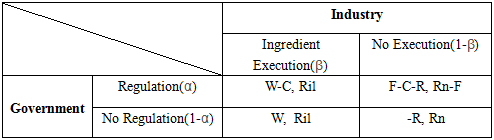
\includegraphics[width=0.5\columnwidth]{figure/result.png}
\label{table:2}
\caption{Table to test captions and labels}
\end{table}
\end{center}

the variables we have defined, we could get the Expectation value of government:

\[
E_{il} = \alpha\beta(W-C) + \alpha(1-\beta)(F-C-R) + (1-\alpha)\beta W + (1-\alpha)(1-\beta)R
\]

Analogously, the Expection value of Industry:

\[
E_c = \alpha\beta R_{il} + \alpha(1-\beta)(R_n-F) + (1-\alpha)\beta R_{il} + (1-\alpha)(1-\beta)R_n
\]

According to the \cite{chenlihong} analysis, we calculate the equilibrium solution for this Game Theory Model, 
and then we get optimal response functions for each entities (Government and Industry).

\begin{equation}
\alpha = \left\{
\begin{array}{ll}
0 & \text{if} \quad \beta > \frac{F-C}{F} \\
\lbrack 0, 1 \rbrack & \text{if} \quad \beta = \frac{F-C}{F} \\
1 & \text{if} \quad \beta < \frac{F-C}{F} \\
\end{array}
\right.
\end{equation}

\begin{equation}
\beta = \left\{
\begin{array}{ll}
0 & \text{if} \quad \alpha < \frac{R_n-R_{il}}{F} \\
\lbrack 0, 1 \rbrack & \text{if} \quad \alpha = \frac{R_n-R_{il}}{F} \\
1 & \text{if} \quad \alpha > \frac{R_n-R_{il}}{F} \\
\end{array}
\right.
\end{equation}


The intersection of two functions is the mixed Nash equilibrium in the government regulation 
during the execution of Ingredient List. Finally we get the unique deterministic solution, that is 

\[
\alpha^* = \frac{R_n - R_{il}}{F}
\]
\[
\beta^* =  \frac{F - C}{F}
\]

which means the Government is intended to regulation the Industries at the probability of $\alpha^*$, 
and the Industry execute Ingredient List at the probability of $\beta^*$, none of them should not 
change this balance state unilaterally, otherwise one of their profits could be damaged.
 
\subsection{Ecosystem of Recycling}
%Maybe picture of this system, if space is required.
% source: Exploring e-waste management systems in the United States
Kahhat et al. proposed a ``deposit-refund system"~\cite{kahhat2008exploring} for the successful collection and 
recycling of e-waste. In this economic system the consumer has to 
``pay a deposit on purchase, a variable portion of which is returned when turned in at the end-of-life"~\cite{plambeck2009effects}. 
The interest collected by this deposit will compensate for overhead costs such as transportation 
and storage fees of recycling-companies. Moreover, as the returned deposit can vary, 
recycling companies with better recycling processes, can offer a higher return to consumers, 
as they will still gain revenue for the resources in recycled products. 
This system does not only ensure the return of e-waste by consumers, 
but also favors companies, who can recycle more effectively.

Wowever, one huge downside of this system is the requirement to track to-be-sold devices, 
as the deposit is linked to the device. With our solution of an ingredient list for 
all released devices  this requirement could be avoided. We would eliminate the deposit 
(and with that the tracking) and collect additional tax, when purchasing electronics. 
Moreover, consumers will be able to sell their e-waste to recycling companies refunding their tax payment in the process. 

Another important advantage of the ingredient list is that, recycling companies know the 
contents of a device and as such could concentrate on specific recycling processes. 
Another weakness of Kahhats et al.'s system~\cite{kahhat2008exploring} is that, a company alone would not 
be able to recycle a product completely - however, recycling companies could negate this 
by selling partly recycled products to each other. The specialized companies, which would 
be possible by the ingredient list, would allow this selling process.

With the collected tax the government could support the establishment of recycling companies 
and in general the ecosystem of recycling dynamically. This offers huge flexibility, which 
is required in the area of electronics, as this market is a ever changing one. With the 
release of ingredient lists, the government can determine, which resources will be needed 
for production and  as a result for recycling. Thus, the government can subsidize effectively and visionary.

To sum up, the ingredient list could eliminate critical weaknesses of Kahhat et al.'s system, 
while also offering new possibilities.


\label{applications}